%%%%%%%%%%%%%%%%%%%%%%%%%%%%%%%%%%%%%%%%%
% Short Sectioned Assignment
% LaTeX Template
% Version 1.0 (5/5/12)
%
% This template has been downloaded from:
% http://www.LaTeXTemplates.com
%
% Original author:
% Frits Wenneker (http://www.howtotex.com)
%
% License:
% CC BY-NC-SA 3.0 (http://creativecommons.org/licenses/by-nc-sa/3.0/)
%
%%%%%%%%%%%%%%%%%%%%%%%%%%%%%%%%%%%%%%%%%

%----------------------------------------------------------------------------------------
%	PACKAGES AND OTHER DOCUMENT CONFIGURATIONS
%----------------------------------------------------------------------------------------

\documentclass[paper=a4, fontsize=11pt]{scrartcl} % A4 paper and 11pt font size

\usepackage[T1]{fontenc} % Use 8-bit encoding that has 256 glyphs
\usepackage{fourier} % Use the Adobe Utopia font for the document - comment this line to return to the LaTeX default
\usepackage[english]{babel} % English language/hyphenation
\usepackage{amsmath,amsfonts,amsthm} % Math packages

\usepackage{lipsum} % Used for inserting dummy 'Lorem ipsum' text into the template
\usepackage{graphicx}

\usepackage{sectsty} % Allows customizing section commands
\allsectionsfont{\centering \normalfont\scshape} % Make all sections centered, the default font and small caps

\usepackage{fancyhdr} % Custom headers and footers
\pagestyle{fancyplain} % Makes all pages in the document conform to the custom headers and footers
\fancyhead{} % No page header - if you want one, create it in the same way as the footers below
\fancyfoot[L]{} % Empty left footer
\fancyfoot[C]{} % Empty center footer
\fancyfoot[R]{\thepage} % Page numbering for right footer
\renewcommand{\headrulewidth}{0pt} % Remove header underlines
\renewcommand{\footrulewidth}{0pt} % Remove footer underlines
\setlength{\headheight}{13.6pt} % Customize the height of the header

\numberwithin{equation}{section} % Number equations within sections (i.e. 1.1, 1.2, 2.1, 2.2 instead of 1, 2, 3, 4)
\numberwithin{figure}{section} % Number figures within sections (i.e. 1.1, 1.2, 2.1, 2.2 instead of 1, 2, 3, 4)
\numberwithin{table}{section} % Number tables within sections (i.e. 1.1, 1.2, 2.1, 2.2 instead of 1, 2, 3, 4)

\setlength\parindent{0pt} % Removes all indentation from paragraphs - comment this line for an assignment with lots of text

%----------------------------------------------------------------------------------------
%	TITLE SECTION
%----------------------------------------------------------------------------------------

\newcommand{\horrule}[1]{\rule{\linewidth}{#1}} % Create horizontal rule command with 1 argument of height

\title{	
\normalfont \normalsize 
\textsc{University of Iowa, Professor Omar Haider} \\ [25pt] % Your university, school and/or department name(s)
\horrule{0.5pt} \\[0.4cm] % Thin top horizontal rule
\huge Databases in OpenEMR \\ % The assignment title
\horrule{2pt} \\[0.5cm] % Thick bottom horizontal rule
}

\author{Junhyuk Kang} % Your name

\date{Oct 11, 2016 ~ Oct 24, 2016 } % Today's date or a custom date


\begin{document}

\maketitle % Print the title

%----------------------------------------------------------------------------------------
%	PROBLEM 1
%----------------------------------------------------------------------------------------
\section{Question}
\begin{enumerate}
  \item What does Comments column on Logdata represent?

\end{enumerate}
%----------------------------------------------------------------------------------------
%	PROBLEM 2
%----------------------------------------------------------------------------------------

\section{Answer Steps}

%------------------------------------------------
\begin{itemize}
	\item Firstly, I thought that the comments number on logdata rerpresents the different user who access to the database
	\item So I tried to start with making several users in different roles
		\begin{itemize}
		\item
		 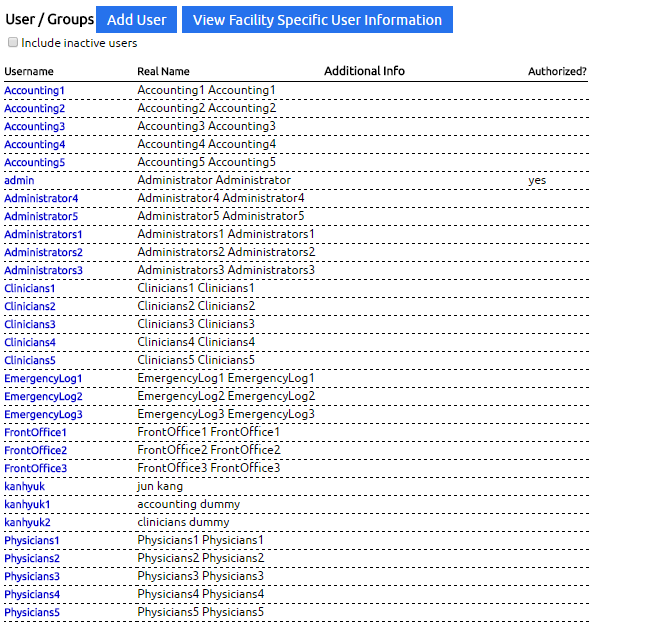
\includegraphics[width = 20cm, height=10cm]{pictures/users.png}
		\end{itemize}
	\item and I found that we have same numbers in same user
	\begin{itemize}
		\item for example, we have both 21 for Physicians2 user, and 20 for FrontOffice1 user
		\item 
		 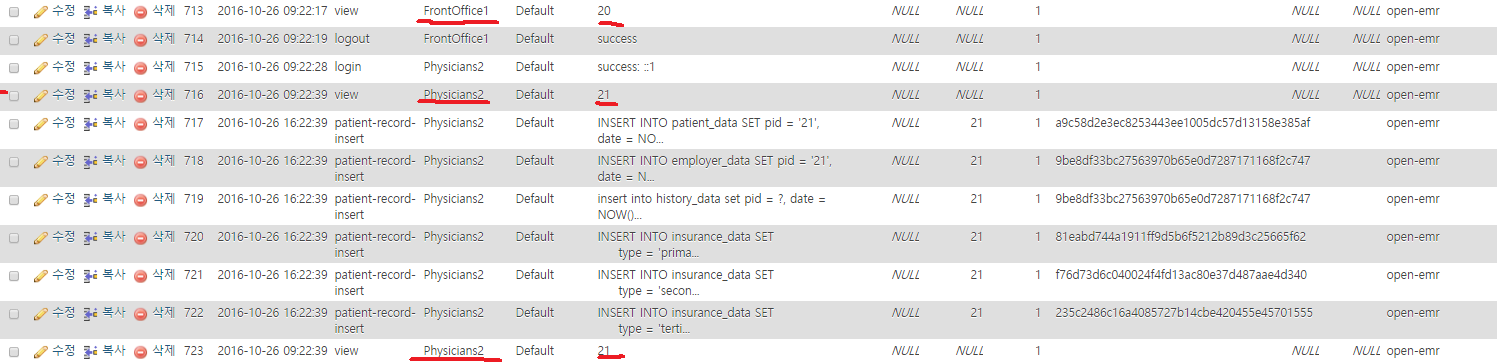
\includegraphics[width = 20cm, height=10cm]{pictures/samenumberinsameuser1.png}
		\end{itemize}
	\item but I found that same user can have different number in comments
	\begin{itemize}
		\item
		 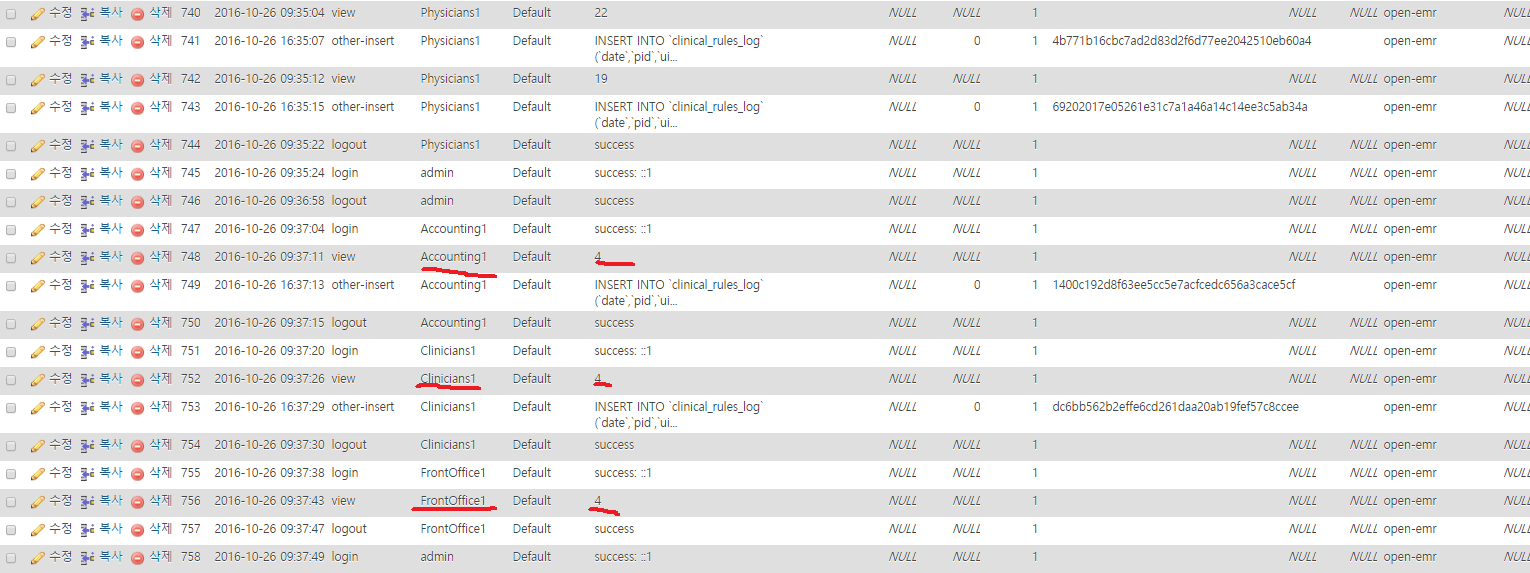
\includegraphics[width = 20cm, height=10cm]{pictures/samenumberinsameaction.png}
		\end{itemize}
	\item So I tried to do same action with different users (I opened 1st patient in patient list)
	\begin{itemize}
		\item
		 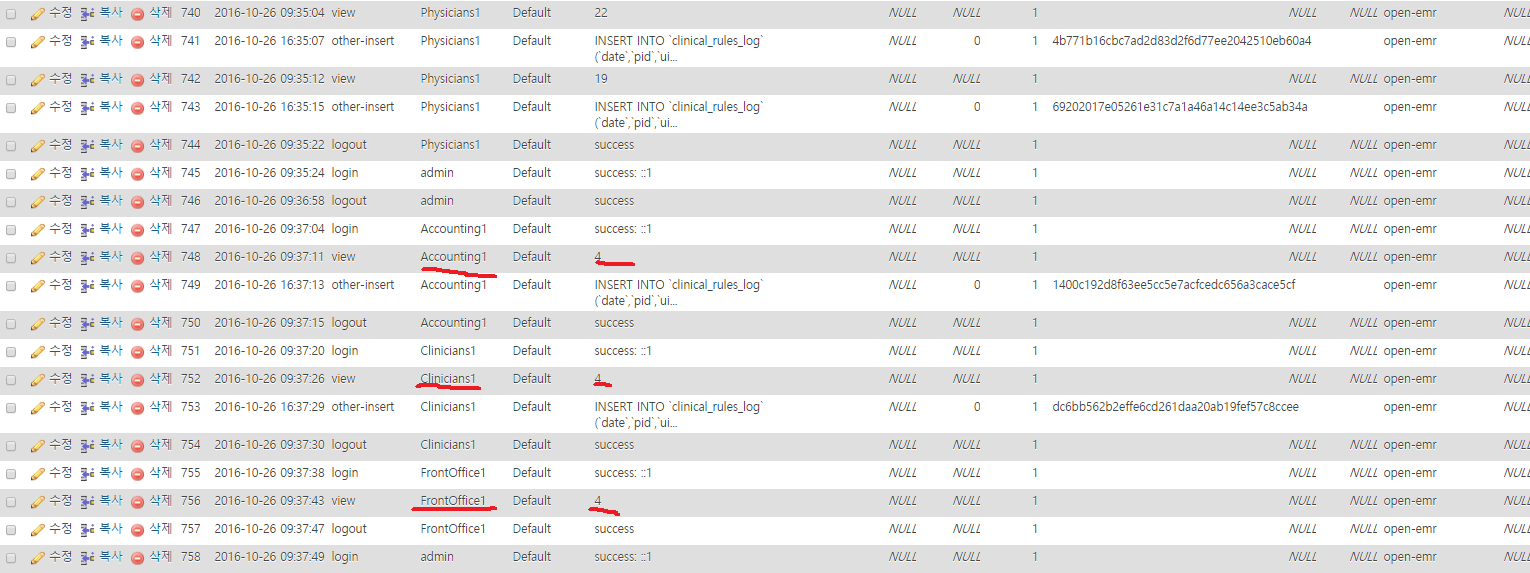
\includegraphics[width = 20cm, height=10cm]{pictures/samenumberinsameaction.png}
		\item and it gives us same number with different users
		\end{itemize}
	\item I changed my hypothesis to that numbers represent each customers
		\begin{itemize}
		\item so I opened several patients with same users(Clinicians3)
		\item
		 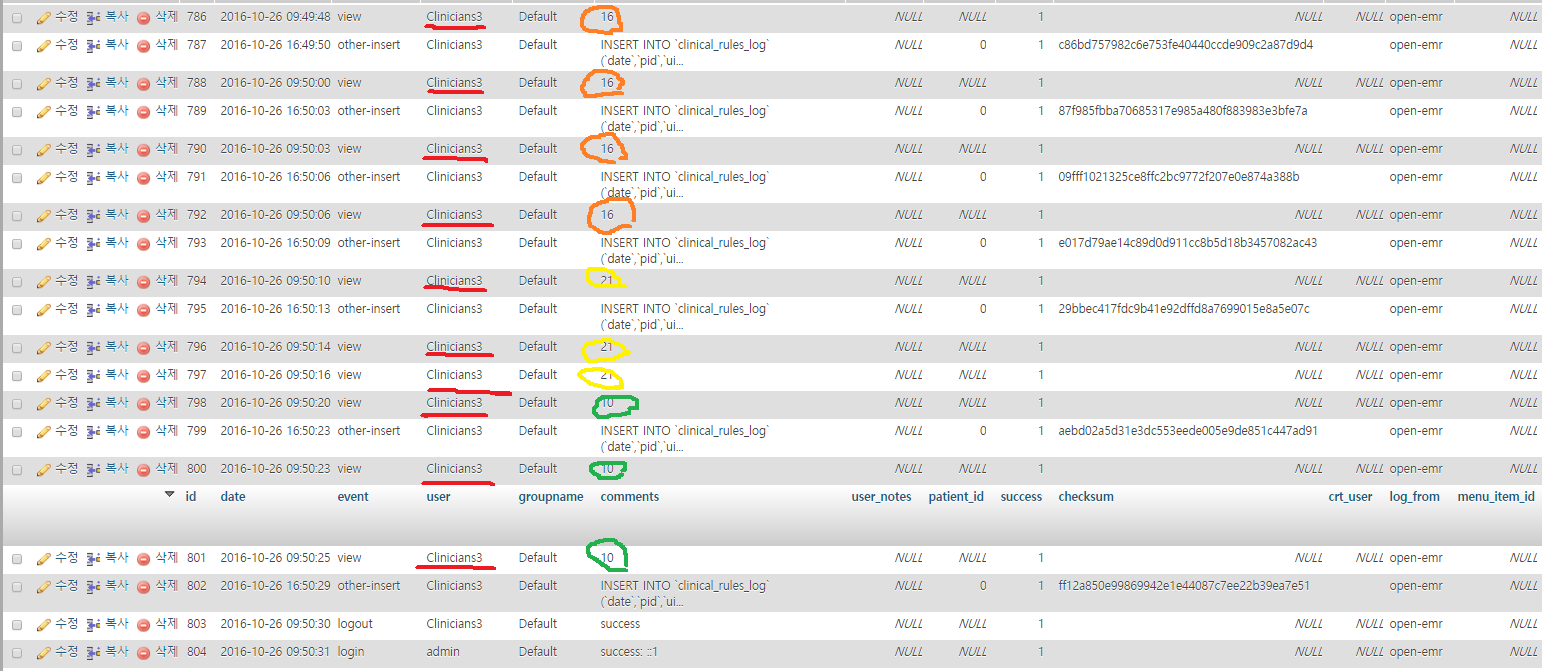
\includegraphics[width = 20cm, height=10cm]{pictures/samenumberinsamepatients.png}
		\item and it gives us different numbers
		\end{itemize}
	\item In conclusion, the comments column in log data represents different patients




				
\end{itemize}












\end{document}